\section{SIMD nodes}

\ac{SIMD} nodes are the main processing cores of the image processor and are
responsible for carrying out data processing-instructions in paralell. They
share the same instruction set and executes the same instruction, hence
\acf{SIMD} and operates on an 8-bit word size, as most of the processor does.

Each \ac{SIMD} node is fully equipped with a register bank, an \ac{ALU}, message
passing with adjacent nodes and an instruction decoder for the \ac{SIMD} node
instruction set, explained in detail in subsequent section.

The schematic of a single \ac{SIMD} node is shown in figure
\ref{fig:fpga-simd-arch} details the entire datapath for the node. Different
parts of the instruction and other inputs and outputs to and from the node are
all labled with red lables. In this section we will reffer to this image when
explaining the different components.

\TODO{Fix signal labels in arhitecture image to differentiate between input, output and instruction}

\begin{figure}[h]
  \centering
 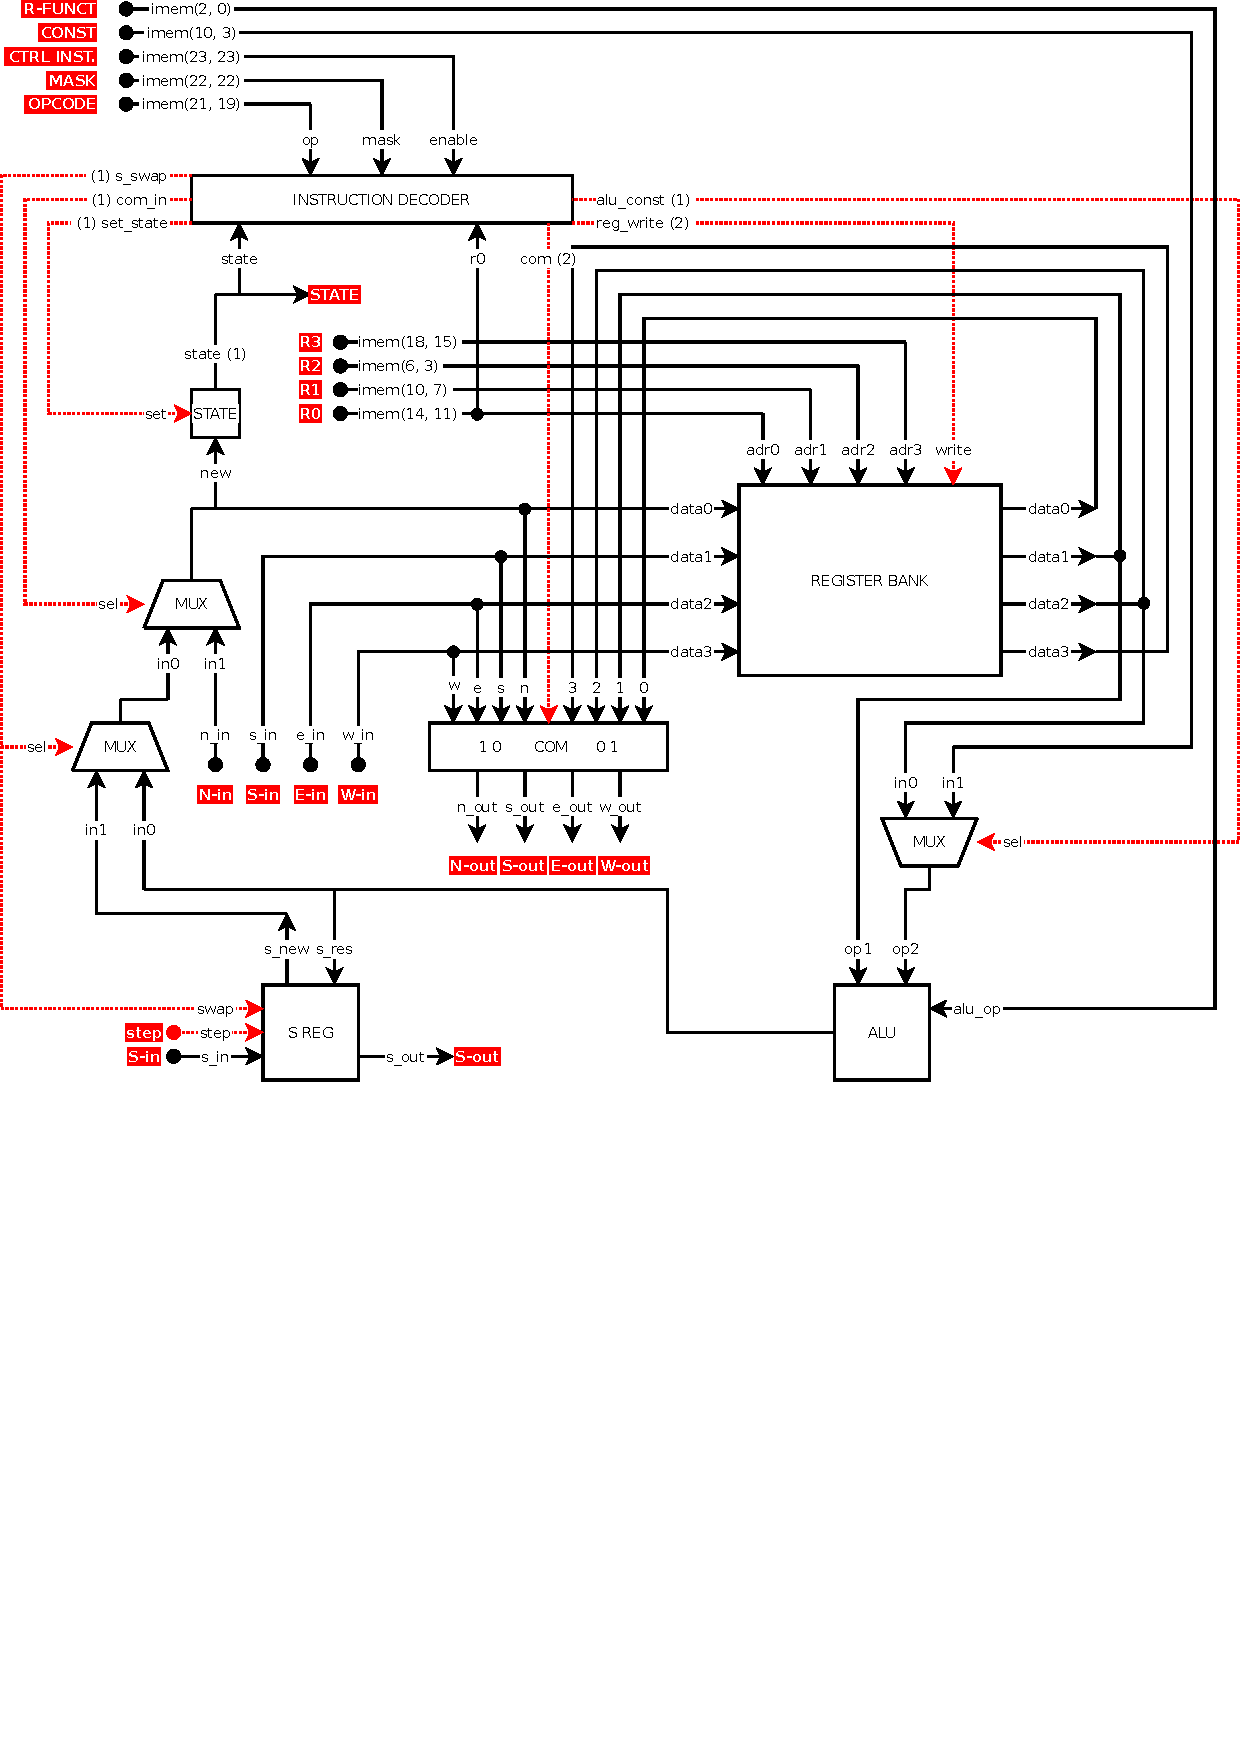
\includegraphics[width=\linewidth,clip,trim=0 0 0 0]
                  {fig/fpga/fpga-simd-arch.pdf}
  \caption{LENA SIMD architecture}
  \label{fig:fpga-simd-arch}
\end{figure}

\TODO{Jahre nevner at det må tydeligjøres hva som er busser og hva som er signaler}

\subsection{Components}

\TODO{This pharagraph is kind of VHDL implementation specific. Should we keep it?}

In order to the keep the ammount of intermediate signals to a minimum, as well
as better reusability accross other parts of the processor, the \ac{SIMD} node
is nicely divided into separate, stand-alone, components which when linked
together makes up the datapath for the node.

\subsubsection{Instruction Decoder}

\TODO{List all the different OP-codes and their meaning.}

When an instructions is first recieved by a \ac{SIMD} node the first 5-bits
(enable, mask and opcode) are fed directly into the Instruction Decoder. The
decoder will then set up the correct control signals other components based on
the current state of the \ac{SIMD} node and instruction opcode.

\subsubsection{Communication}
The Communication component controlls outbound data from the \ac{SIMD} node to
adjacent \ac{SIMD} nodes in the grid array. It can either send data from 4
registers out on north-, south-, east- and west-bound links, forward incoming
links in an clockwise spiral according to \ref{fig:fpga-simd-datacom} or keep
the previously outgoing data. The latter is very important in order for
branching to work correctly; where some \ac{SIMD} nodes, depending on their
state, may store incoming data in one register and others \ac{SIMD} nodes in an
other register.

The clockwise spiral forwarding is an optimized way of distributing a 3x3 array
of source data to all the \ac{SIMD} nodes in the grid array using only 3-clock
cycles. \TODO{We made this one ourselves! note that down}
\TODO{Jahre vil at dettte skal forklares bedre}

\subsubsection{Register Bank}
Each \ac{SIMD} node is equpped with $2^4 = 16$ general purpose registers. 14 of
which are available for general storage during acecution. The remaining 2 are
reserved for the special purpose registers {\tt \$zero} and {\tt \$state}.

\begin{table}[h]
  \centering
  \begin{tabularx}{\linewidth}{XXXXXXXXX}\toprule
    R0 & R1 & R2 & R3 & R4 & R5 & R6 & R7 \\ \midrule
    \tt \$zero & \tt \$r1 & \tt \$r2 & \tt \$r3 & \tt \$r4 & \tt \$r5 &
    \tt \$r6 & \tt \$r7\\ \bottomrule
  \end{tabularx}
  \begin{tabularx}{\linewidth}{XXXXXXXX}
    R8 & R9 & R10 & R11 & R12 & R13 & R14 & R15 \\ \midrule
    \tt \$r8 & \tt \$r9 & \tt \$r10 & \tt \$r11 & \tt \$r12 & \tt \$r13 &
    \tt \$r14 & \tt \$state\\ \bottomrule
  \end{tabularx}
  \caption{Registers in the SIMD nodes}
  \label{tab:simd-registers}
\end{table}


The register bank has specially designed with the four way data transfer in
mind. It supports reading, or writing, 4 registers at once or reading 2
registers and writing 1 register within one clockcycle.

\subsubsection{Arithmetic Logic Unit}

\TODO{List the 8 ALU functions somewhere with their binary prepresentation.}

The \ac{ALU} implemented is a very simple {\tt 8}-bit \ac{ALU} supporting only 8
instructions. The main reason for only implementing the most basic arithmetic
instruction was to save space in the instruction set, since all \ac{SIMD} node
instructions carries the 3-bit \ac{ALU} function at the end, and to reduce the
pysical size of the node.

\TODO{Add some supporting references.}

Upon investigating image processing algorithmes we found that many of these,
Median Filter and Salt and Pepper noise reduction, only need these 8 \ac{ALU}
operations in order to perform their work. Besides; more high level arithmetic,
such as multiply and divide, can be implemented using addition and subtraction.
\TODO{Jahre skriver: "2 Er ikke mange. Hvilke andre har dere kikket på?"}
\subsubsection{Source Data Register}
The source data register (S REG), is a special purpose register within the
\ac{SIMD} node which holds the next source data for the \ac{SIMD} node. It is
partly controlled by the \ac{SIMD} node instruction set and partly by a special
{\tt step} signal sent from the \ac{DMA}.

An important attribute of the S REG is its capability to receive data from the
left node and passing it along to node on the right when instructed by the {\tt
  step} signal. This allows for a simultaneous data transfer while the node is
otherwise busy processing.

\subsubsection{State Register}
In order to handle branches the \ac{SIMD} node must have some internal
state. The State Register is, as all other registers, 8-bit. The least
significant bit is the current state wich is sent out from the node and to the
Instruction Decoder unit within the \ac{SIMD} node.

The State Register can be written and read as any other register in the Register
Bank and the state can hence be shifted left or right in order to acheave nested
branches.

\subsection{DRAM and SRAM}

\TODO{Where to put this?}

\ac{DRAM} or \ac{SRAM} is not available from the \ac{SIMD} nodes.

\subsection{Instruction Set}

\begin{figure}[h]
  \centering
  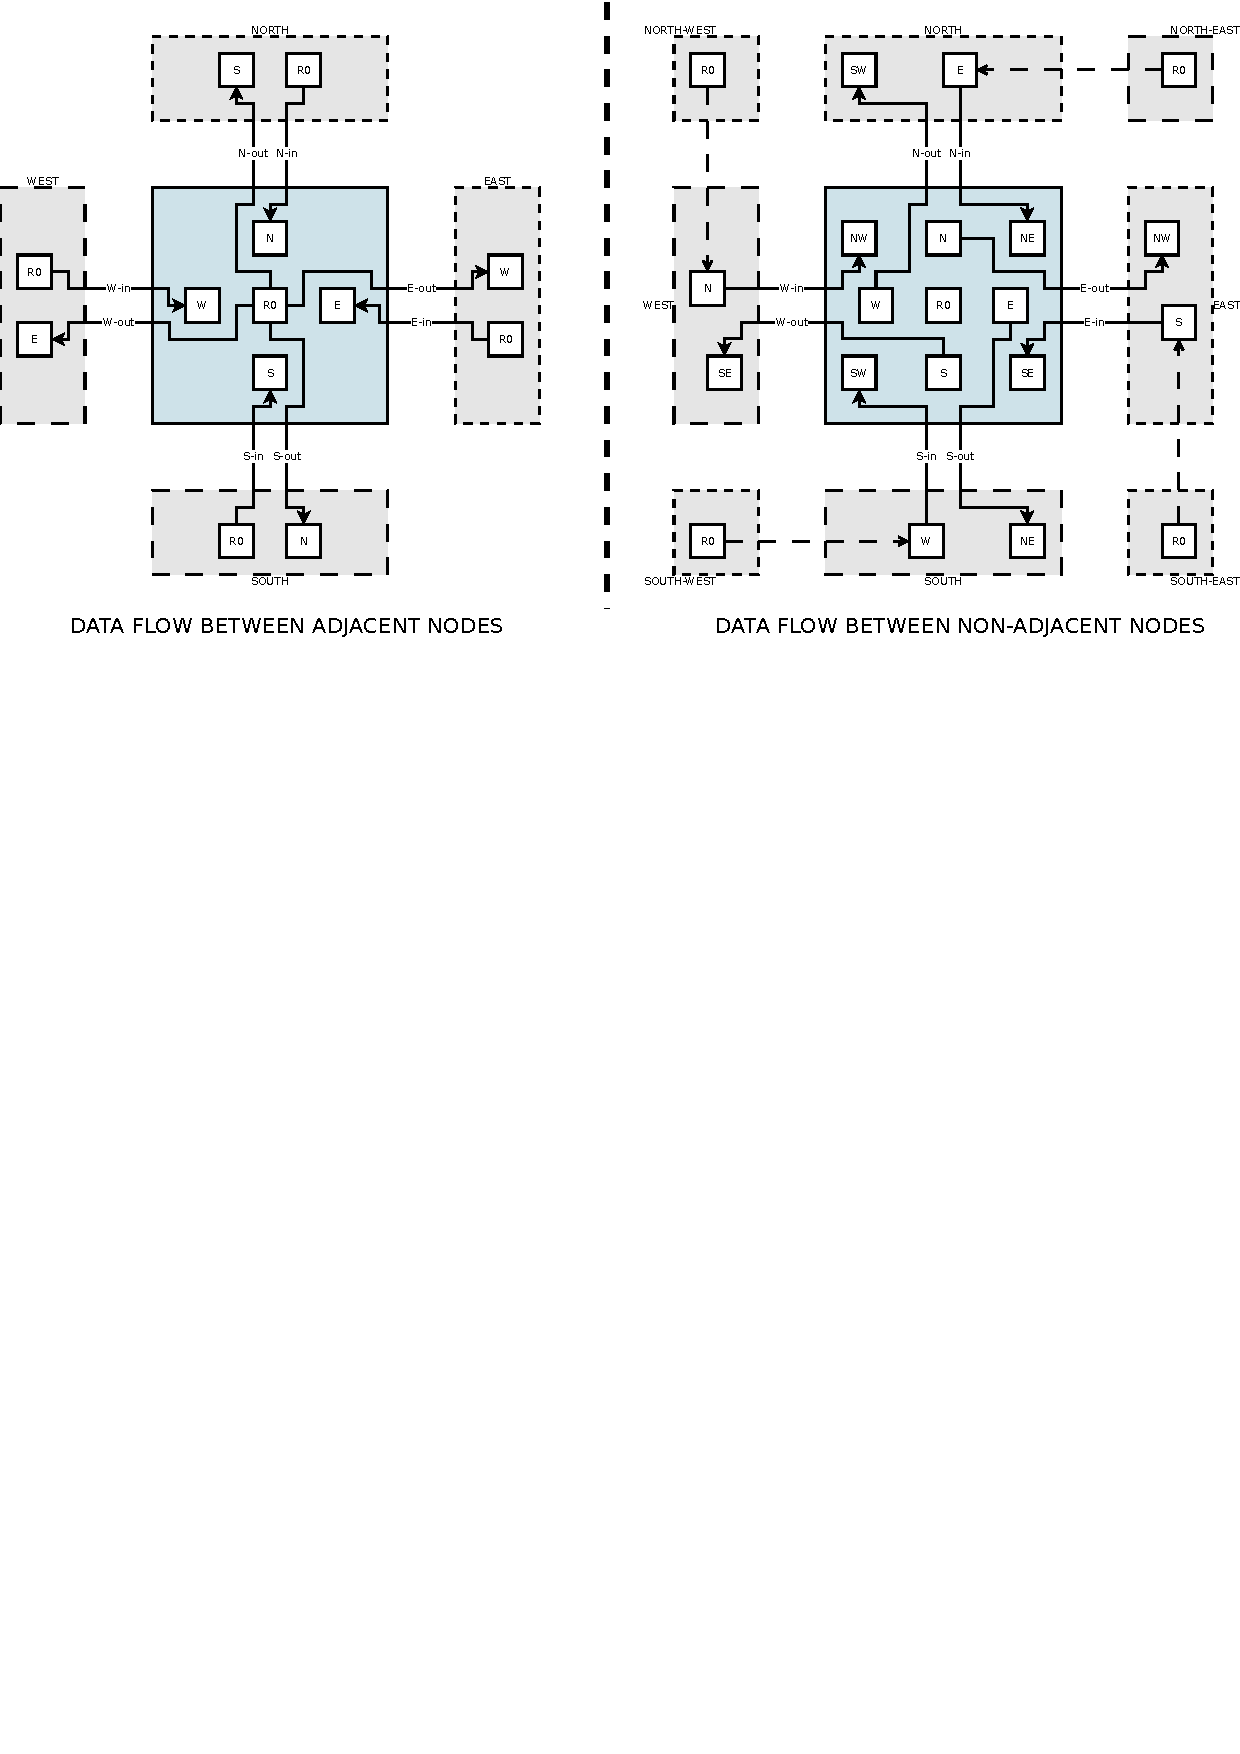
\includegraphics[width=\linewidth,clip,trim=0 18cm 0 0]
                  {fig/fpga/fpga-simd-datacom.pdf}
  \caption{Four-way communication in the LENA SIMD array.}
  \label{fig:fpga-simd-datacom}
\end{figure}


\subsection{Branching}
\CHECK{Should this be added to the appendix or something?}

Since all nodes run the same instructions, both parts of a branch must be
executed. Nodes are setting the {\tt state} to 1 in order to indicate that they
are executing within that part of the branch.

\begin{table}[h]
  \centering
  \begin{tabularx}{\textwidth}{rlcX}\toprule
    \thxc{step} & \thxc{instruction} & \thxc{state} & \thxc{description} \\
    \midrule
    0 & \tt // initial state & 0 & \\
    1 & \tt eq \$state \$r1, \$r2 & 1
    & Set state to 1 if branch should be taken for the node.\\
    \ldots & \tt // branch taken & 1 &
    Instructions for when the branch is taken.\\
    2 & \tt eq \$state, \$state, \$zero & 0 & Negate the state.\\
    \ldots & \tt // branch not taken & 0 & Instructions for when the branch is
    not taken.\\ \bottomrule
  \end{tabularx}
  \caption{Single level branching}
  \label{tab:single-level-branching}
\end{table}


\subsubsection{Multilevel branching}
Since state register is 8 it is possible to have up-to 8 nested branches by
shifting the current state to the left and adding the new state to the
end. Below \TODO{Refer to table, not relative to where it is placed} are the
instructions for performing a multilevel-branch.

\CHECK{Better switch out zeroes and ones with x'es and y's?}
\begin{table}[h] % TODO: Drag out
  \centering
  \begin{tabularx}{\textwidth}{rlcX}\toprule
    \thxc{step} & \thxc{instruction} & \thxc{state} & \thxc{description} \\
    \midrule
    0 & \tt // initial state & 01 & \\
    1 & \tt sll \$r3, \$state & 01
    & Save the current state by shifting left.\\
    2 & \tt eq \$r4 \$r1, \$r2 & 01
    & Calculate if branch is taken for the node.\\
    3 & \tt add \$state \$r4, \$r3 & 11
    & Set the new state.\\
    \ldots & \tt // branch taken & 11 &
    Instructions for when the branch is taken.\\
    4 & \tt andi \$r3, \$state, 1111 1110 & 11
    & Save the old state for the node.\\
    5 & \tt andi \$r4, \$state, 0000 0001 & 11 & Save the current state.\\
    6 & \tt eq \$r4, \$r4, \$zero & 11 & Negate the current state.\\
    7 & \tt add \$state, \$r4, \$r3 & 10 & Set new state.\\
    \ldots & \tt // branch not taken & 10
    & Instructions for when the branch is not taken.\\
    8 & \tt srl \$state, \$state & 01 & Revert to state before branch by
    shifting right.\\ \bottomrule
  \end{tabularx}
  \caption{Multi level branching}
  \label{tab:multi-level-branching}
\end{table}

\CHECK{Could any of these tables be figures instead?}
